%TODO Why is the global status relevant
%Is there other things that should be described in the report

\section{State Machine}
The watchdog manager has a state machine \ref{FIG:GLOBALSTATUSES},
which transitions depend on the on global variables, changes of global
variables, and the current state. If the behavior of the watchdog manager is
correct and the manager is actually running, or in other words not deactivated,
it stays in 'WDGM\_GLOBAL\_STATUS\_OK'. There are however lots of reasons for
that the status will change from the correct state. It depends on arguments to
the API calls but also in which order commands are called. Also the supplied
AUTOASAR configuration is relevant, because it specifies tolerances of faulty
behavior, it may indirectly disable some states and state transition or make some
transition more likely to happen. The effect can for instance come from
the number of checkpoints supplied in the configuration. A correct behavior of
the watchdog manager depends on that checkpoints are reached and does so in the
right order.

The only function that can change the global status is the main function. The
main function is continuously called in a given time interval, note that the
timing is not used when using quickcheck \ref{SEC:CALLING_COMMANDS}, schedule be
the run time environment (RTE).


\begin{figure}[h!]
\label{FIG:GLOBALSTATUSES}
\caption{State diagram that shows possible trasitions between states}
\begin{center}
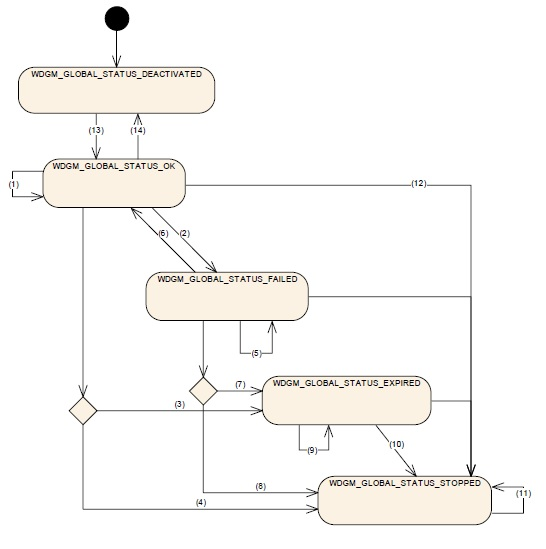
\includegraphics{pictures/globalstatuses.jpg}
\end{center}
\end{figure}



\section{Configurations}
The WdgM was tested using three different configurations.
% Which are they and why were they chosen

\subsection{BSI}
A highly simplified configuration \emph{BSI} gives in some sense good results.
Using this configuration the WdgM was never hitting the absorbing state
according to \ref{FIG:GLOBALSTATUSES}.  However looking at the state
transitions, comparing figure \ref{FIG:GLOBALSTATUSES} and table
\ref{TABLE:STATUSES_BSI}, only two states are hit. This happens
because the configuration is to simply, it is actually impossible to hit
any other states then \emph{'GLOBAL\_STATUS\_OK'} or
\emph{'GLOBAL\_STATUS\_DEACTIVATED'}. There are no checkpoints or supervision
algorithms configured for the \emph{BSI} configuration.
Hence it is easy to run tests using this configuration but it does, by it self,
not fully test the code because some specification requirements will never be
tested. The untested requirements are mainly requirements for supervision algorithms
that are, according to the configuration, never supposed to be run. Those
untested requirements leaves also other requirements untested because
the watchdog manager never reaches a state when those other requirements must hold.
\begin{figure}[h!]
\label{FIG:BSI}
\caption{BSI configuration}
\begin{center}
\subfigure[Shows percentage of each possible command executed]{
\label{FIG:COMMANDS_BSI}
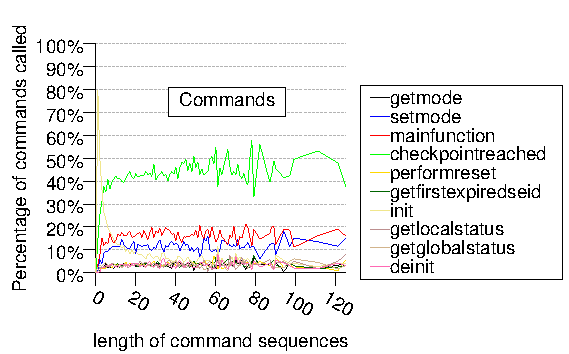
\includegraphics{generated_pictures/history_commands_bsi.pdf}
}

\subfigure[Shows percentage of each possible global status hit]{
\label{FIG:STATUSES_BSI}
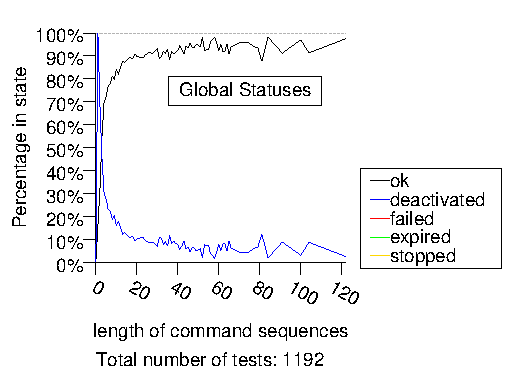
\includegraphics{generated_pictures/history_statuses_bsi.pdf}
}
\end{center}
\end{figure}

\begin{table}[h!]
\label{TABLE:STATUSES_BSI}

    \begin{tabular}{r|ccccc}
        \hline
        \multicolumn{6}{c}{Number of tests: 2850} \\
        \hline
        \backslashbox{From}{To}
                    & DEACTIVATED & EXPIRED & FAILED & OK & STOPPED \\
        \hline
        DEACTIVATED & \bf{02.23}\% & 00.00\%       & 00.00\%       & \bf{09.12}\% & 00.00\% \\
        EXPIRED     & 00.00\%       & \bf{00.00}\% & 00.00\%       & 00.00\%       & \bf{00.00}\% \\
        FAILED      & 00.00\%       & \bf{00.00}\% & \bf{00.00}\% & \bf{00.00}\% & \bf{00.00}\% \\
        OK          & \bf{03.24}\% & \bf{00.00}\% & \bf{00.00}\% & \bf{85.41}\% & \bf{00.00}\% \\
        STOPPED     & 00.00\%       & 00.00\%       & 00.00\%       & 00.00\%       & \bf{00.00}\%
      \end{tabular}
    

\caption{bsi configuration}
\end{table}

\subsection{freescale}
The freescale configuration is, compared to BSI, a more realistic configuration.
All supervision algorithms are configured and there are both external and
internal graphs for logical supervision. It is also the configuration, mainly
used at Mecel. The state machine for the global status is totally covered by
running QuickCheck, see table \ref{TABLE:STATUSES_FREESCALE} and figure \ref{FIG:GLOBALSTATUSES}.  


\begin{figure}[h!]
\label{FIG:FREESCALE}
\caption{Freescale configuration}
\begin{center}

\subfigure[Shows percentage of each possible command executed]{
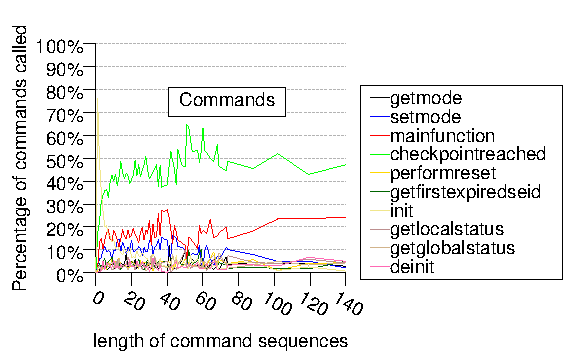
\includegraphics{generated_pictures/history_commands_freescale.pdf}
\label{FIG:COMMANDS_FREESCALE}
}
\subfigure[Shows percentage of each possible global status hit]{
\label{FIG:STATUSES_FREESCALE}
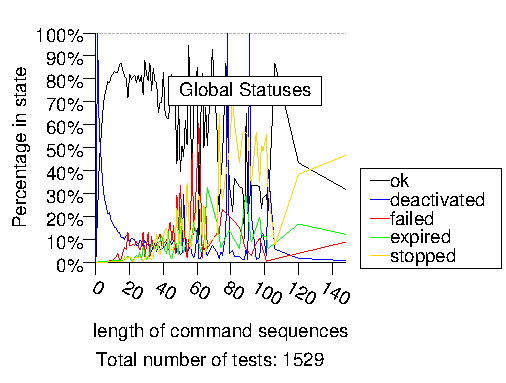
\includegraphics{generated_pictures/history_statuses_freescale.pdf}
}
\end{center}
\end{figure}

\begin{table}[!h]
\label{TABLE:STATUSES_FREESCALE}

    \begin{tabular}{r|ccccc}
        \hline
        \multicolumn{6}{c}{Number of tests: 1023} \\
        \hline
        \backslashbox{From}{To}
                    & DEACTIVATED & EXPIRED & FAILED & OK & STOPPED \\
        \hline
        DEACTIVATED & \bf{02.43}\% & 00.00\%       & 00.00\%       & \bf{08.32}\% & 00.00\% \\
        EXPIRED     & 00.00\%       & \bf{03.36}\% & 00.00\%       & 00.00\%       & \bf{00.11}\% \\
        FAILED      & 00.00\%       & \bf{00.17}\% & \bf{07.77}\% & \bf{00.12}\% & \bf{00.11}\% \\
        OK          & \bf{02.56}\% & \bf{00.18}\% & \bf{00.87}\% & \bf{69.53}\% & \bf{00.12}\% \\
        STOPPED     & 00.00\%       & 00.00\%       & 00.00\%       & 00.00\%       & \bf{04.34}\%
      \end{tabular}
    

\caption{freescale configuration}
\end{table}

\subsection{example}

\begin{figure}[h!]
\caption{Example configuration}
\label{FIG:EXAMPLE}
\begin{center}

\subfigure[Shows percentage of each possible command executed]{
\label{FIG:COMMANDS_EXAMPLE}
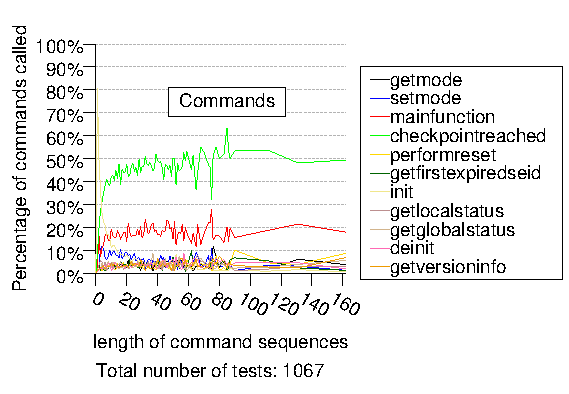
\includegraphics{generated_pictures/history_commands_example.pdf}
}

\subfigure[Shows percentage of each possible global status hit]{
\label{FIG:STATUSES_EXAMPLE}
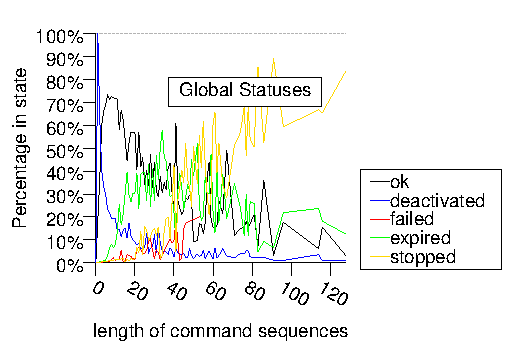
\includegraphics{generated_pictures/history_statuses_example.pdf}
}

\end{center}
\end{figure}

\begin{table}[!h]
\label{TABLE:STATUSES_EXAMPLE}

    \begin{tabular}{r|ccccc}
        \hline
        \multicolumn{6}{c}{Number of tests: 3877} \\
        \hline
        \backslashbox{From}{To}
                    & DEACTIVATED & EXPIRED & FAILED & OK & STOPPED \\
        \hline
        DEACTIVATED & \bf{02.59}\% & 00.00\%       & 00.00\%       & \bf{07.81}\% & 00.00\% \\
        EXPIRED     & 00.00\%       & \bf{24.77}\% & 00.00\%       & 00.00\%       & \bf{00.81}\% \\
        FAILED      & 00.00\%       & \bf{00.12}\% & \bf{02.87}\% & \bf{00.00}\% & \bf{00.04}\% \\
        OK          & \bf{01.68}\% & \bf{02.50}\% & \bf{00.39}\% & \bf{40.22}\% & \bf{00.14}\% \\
        STOPPED     & 00.00\%       & 00.00\%       & 00.00\%       & 00.00\%       & \bf{16.07}\%
      \end{tabular}
    

\caption{example configuration}
\end{table}

\section{Handle bugs in the C code}
\label{sec:handlebugs}

\section{Functional safety analysis}
\subsection{Definition of time}
\label{SEC:FUNCTIONAL_SAFETY_TIME}

\section{Statistics}
